% To je predloga za poročila o domačih nalogah pri predmetih, katerih
% nosilec je Tomaž Curk. Avtor predloge je Blaž Zupan.
%
% Seveda lahko tudi dodaš kakšen nov, zanimiv in uporaben element,
% ki ga v tej predlogi (še) ni. Več o LaTeX-u izveš na
% spletu, na primer na http://tobi.oetiker.ch/lshort/lshort.pdf.
%
% To predlogo lahko spremeniš v PDF dokument s pomočjo programa
% pdflatex, ki je del standardne instalacije LaTeX programov.

\documentclass[a4paper,11pt]{article}
\usepackage{a4wide}
\usepackage{fullpage}
\usepackage[utf8x]{inputenc}
\usepackage[slovene]{babel}
\selectlanguage{slovene}
\usepackage[toc,page]{appendix}
\usepackage[pdftex]{graphicx} % za slike
\usepackage{setspace}
\usepackage{multicol}
\usepackage{color}
\definecolor{light-gray}{gray}{0.95}
\usepackage{listings} % za vključevanje kode
\usepackage{minted} % za barvanje kode
\usepackage{hyperref}
\renewcommand{\baselinestretch}{1.2} % za boljšo berljivost večji razmak
\renewcommand{\appendixpagename}{Priloge}

\lstset{% nastavitve za izpis kode, sem lahko tudi kaj dodaš/spremeniš
    language=Python,
    basicstyle=\footnotesize,
    basicstyle=\ttfamily\footnotesize\setstretch{1},
    backgroundcolor=\color{light-gray}
}

\newminted{json}{
  % remove first 2 characters (padding spaces)
  gobble = 4,
  % set left line (code block padding hack)
  frame = leftline,
  % 0 width for frame ruler (gives padding but is invisible)
  framerule = 0pt,
  % distance between frame and content
  framesep = 8pt,
  % set background
  bgcolor = light-gray
}

\title{\huge{Vmesno poročilo} \\ \Large{\em{Mreže v socialnem omrežju Vine}}}
\author{Marko Grešak (63130058)}
\date{\today}

\begin{document}

\maketitle

\section{Uvod}

% Tema je zelo zanimiva. Podatki zgledajo zelo bogati. Glavno vprašanje je, ali lahko poiščemo skupnosti v takšnem grafu sodelovanja pri videoposnetkih. Zanimivo bi bilo tudi videti, kako se spreminja časovna dinamika sodelovanja. Kako so s tem povezane oznake (hashtagi). So določena sodelovanja med uporabniki vezana na konkretne hashtage? Kako so hashtagi povezani z gledanostjo. Kakšen je vpliv posameznikov na popularnost videa? So določeni posamezniki tisti, ki nekako zagotovijo uspešnost (gledanost) ali je za to pomembno kaj drugega?

V svoji projektni nalogi analiziram podatke aplikacije oziroma socialnega omrežja
\href{https://vine.co}{\underline{Vine}}. Poizkušam pridobiti čimbolj zanimive
podatke ter jih prikazati na zanimiv način, pri tem pa iščem načine, kako kar se
da dobro prikazati sodelovanje avtorjev ter kakšne skupnosti tvorijo. Pri svoji
raziskavi sem ugotovil, da še nihče ni delal podobne raziskave.

\subsection{Kaj je Vine?}

Ko govorim o projektu se v večini primerov najprej pojavi vprašanje:
\textit{“Kaj je Vine?”}. Vine je Twitterjeva spletna storitev, ki uporabnikom
omogoča nalaganje do 7 sekundnih videov, s časom pa so ga uporabniki začeli
uporabljati kot čisto neodvisno socialno omrežje. Omrežje je postalo popularno
zaradi avtorjev, ki ustvarjajo smešno vsebino, teh pa je iz dneva v dan več, kar
pomeni več podatkov za mojo nalogo.

\section{Podatki}

Med iskanem podatkov nisem našel nobene uporabne povezave, kjer bi bili kakšni
podatki že na voljo. To pomeni, da vse svoje podatke črpam zgolj iz
\href{https://api.vineapp.com}{\underline{Vine API}}.

\subsection{Vine API}

Postopek črpanja podatkov iz APIja se je izkazal za zelo zahtevnega, saj ni
nikakršne uradne dokumentacije, obstaja samo
\href{https://github.com/starlock/vino/wiki/API-Reference}{\underline{Vine API
Reference}}, pa še ta je zastarela, od objave so je format podatkov že
spremenil, povezave pa so na srečo ostale enake.

\subsection{Prijava}

Za dostop do nekaterih podatkov je potreba prijava. Za prijavo pošljemo
\texttt{POST} zahtevo s form podatki

\begin{jsoncode}
    {
        "username": "uporabnisko ime / email",
        "password": "geslo"
    }
\end{jsoncode}

na naslov

\begin{lstlisting}
    https://api.vineapp.com/users/authenticate
\end{lstlisting}

Odgovor na uspešno prijavo pa je JSON objekt s statusom, če je le-ta uspešen pa tudi s podatki o pravkar prijavljenem uporabniku ter ključ seje, ki jo uporabljamo za avtentikacijo pri sledečih poizvedbah.

\subsection{Poizvedbe}

\subsubsection{Popular Now}

API omogoča prikaz popularnih Vinov, ki jih lahko najdemo na strani \href{https://vine.co/popular-now}{\underline{Popular Now}}. Podatke dobimo z \texttt{GET} zahtevo na naslov

\begin{lstlisting}
https://api.vineapp.com/timelines/popular
\end{lstlisting}

\noindent
Rezultati pa niso dokaj zanesljivi, saj so popularni Vini zelo dinamični, saj lahko pri dveh zahtevah z zelo majhno razliko (nekaj sekund) dobimo v odgovor povsem druge Vine.

\subsubsection{Iskanje uporabnikov}

Uporabnike lahko iščemo po uporabniškem imenu. Podatke dobimo z \texttt{GET} zahtevo na naslov

\begin{lstlisting}
https://api.vineapp.com/users/search/<username>
\end{lstlisting}
\noindent
Odgovor pa je seznam najdenih uporabnikov. Na žalost na tem seznamu ni navedenih nobenih zanimivih števil, ko npr. število sledilcev ali objavljenih Vinov. Pridobimo pa id uporabnika, s katerim naredimo še eno poizvedbo, da dobimo podatke o profilu.

\subsubsection{Uporabnikov profil}

Da pridobimo profil uporabnika, potrebujemo id številko uporabnika, eden od načinov je, da ga pridobimo z iskanjem po uporabniškem imenu, seveda če ga poznamo. Da pridobimo profil uporabnika, naredimo \texttt{GET} zahtevo na naslov

\begin{lstlisting}
https://api.vineapp.com/users/profiles/<userid>
\end{lstlisting}
\noindent
Kot odgovor pa dobimo zanimive podatke, kot so lokacija, število sledilcev in število seledenih uporabnikov.

\subsubsection{Uporabnikova časovnica}

Uporabnikova časovnica je najbolj zanimiv del, saj vsebuje vse njihove Vine, iz katerih zbiram podatke ter sledim povezavam med uporabniki. Za dostop do podatkov prav tako potrebujemo id uproabnika, za podatke pa \texttt{GET} zahtevo naslovimo na naslov

\begin{lstlisting}
https://api.vineapp.com/timelines/users/<userid>
\end{lstlisting}
\noindent
Kot odgovor pa dobimo seznam vseh objav Vinov, organiziranih kot strani, npr. 20 Vinov na eno stran.

\section{Vizualizacije}

V času pisanja tega poročila mi ni uspelo izdelati veliko vizualizacij, saj še nisem uspel zbrati zadosti podatkov, da bi jih ustrezno povezal, imam pa dosti zamisli kako bi jih predstavil, poleg tega pa nimam še zadostnega znanja o granjenju in povezovanju uporabnikov v mreže.

\subsection{Ideje}

Najbolj zanimiva mi je predstavitev z grafom sil, kjer jakost sile predstavlja število sodelovanj med dvema uporabnikoma.

\begin{figure}[htbp]
\begin{center}
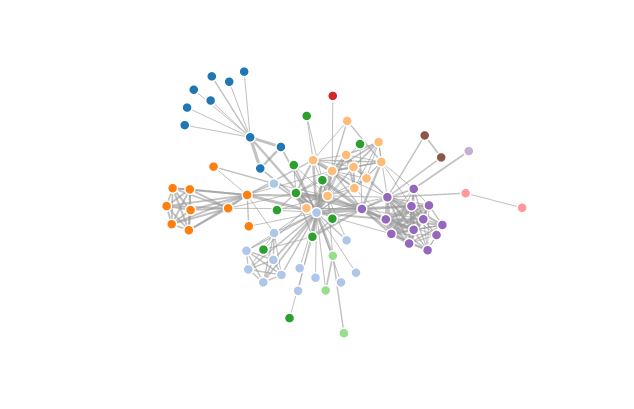
\includegraphics[scale=0.3]{graf.png}
\caption{Graf sil. \textit{(Slika je simbolična)}}
\label{slika1}
\end{center}
\end{figure}

\end{document}
